\documentclass[a4paper,10pt]{article}

\usepackage{listings}
\usepackage[pdftex]{graphicx}
\title{Database fundementals final project}
\author{Name and student number}
\date{23 March 2014}

\begin{document}
\section {Question 4}
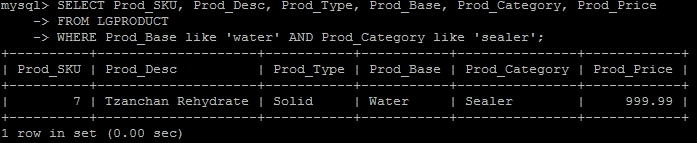
\includegraphics{Queries/Question_4/Q4_screenshot.jpg}
\lstset{
            language=SQL,
            breaklines=true
            }
        \begin{lstlisting}[frame=single]
        SELECT Prod_SKU, Prod_Desc, Prod_Type, Prod_Base, Prod_Category, Prod_Price
FROM LGPRODUCT
WHERE Prod_Base like 'water' AND Prod_Category like 'sealer';

        \end{lstlisting}
\section {Question 5}
\lstset{
            language=SQL,
            breaklines=true
            }
        \begin{lstlisting}[frame=single]
        SELECT Emp_Fname, Emp_Lname, Emp_Email
FROM LGEMPLOYEE
WHERE (Emp_Hiredate BETWEEN '2010-01-01' AND '2013-12-31')
ORDER BY Emp_Lname, Emp_Fname;

        \end{lstlisting}
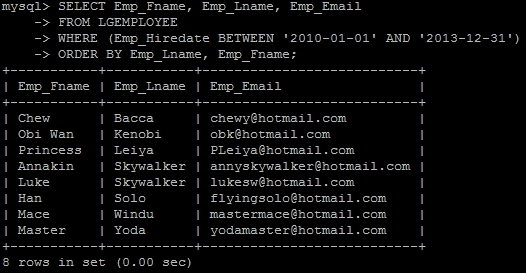
\includegraphics{Queries/Question_5/Q5_screenshot.jpg}
\section {Question 6}
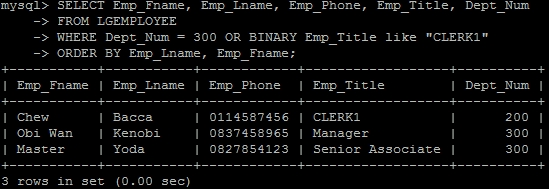
\includegraphics{Queries/Question_6/Q6_screenshot.jpg}
\lstset{
            language=SQL,
            breaklines=true
            }
        \begin{lstlisting}[frame=single]
        SELECT Emp_Fname, Emp_Lname, Emp_Phone, Emp_Title, Dept_Num
FROM LGEMPLOYEE
WHERE Dept_Num = 300 OR BINARY Emp_Title like "CLERK1"
ORDER BY Emp_Lname, Emp_Fname;

        \end{lstlisting}
\section {Question 7}
\lstset{
            language=SQL,
            breaklines=true
            }
        \begin{lstlisting}[frame=single]
        SELECT LGEMPLOYEE.Emp_Num, LGEMPLOYEE.Emp_Lname, LGEMPLOYEE.Emp_Fname, LGSALARY_HISTORY.Sal_From, LGSALARY_HISTORY.Sal_End, LGSALARY_HISTORY.Sal_Amount
FROM LGEMPLOYEE INNER JOIN LGSALARY_HISTORY ON LGEMPLOYEE.Emp_Num=LGSALARY_HISTORY.Emp_Num
WHERE LGEMPLOYEE.Emp_Num = 83731 OR LGEMPLOYEE.Emp_Num = 83745 OR LGEMPLOYEE.Emp_Num = 84039
ORDER BY LGEMPLOYEE.Emp_Num, LGSALARY_HISTORY.Sal_From;

        \end{lstlisting}
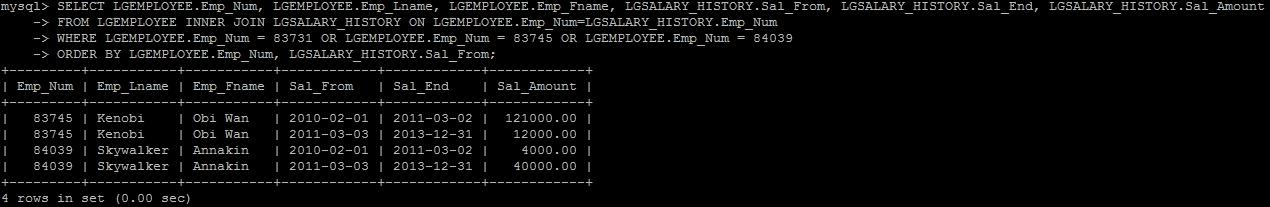
\includegraphics{Queries/Question_7/Q7_screenshot.jpg}
\section {Question 8}
\lstset{
            language=SQL,
            breaklines=true
            }
        \begin{lstlisting}[frame=single]
        SELECT DISTINCT LGCUSTOMER.Cust_Fname, LGCUSTOMER.Cust_Lname, LGCUSTOMER.Cust_Street, LGCUSTOMER.Cust_City, LGCUSTOMER.Cust_Province, LGCUSTOMER.Cust_Zip
FROM LGCUSTOMER, LGBRAND, LGINVOICE, LGPRODUCT
WHERE LGBRAND.Brand_Name like 'Tatooine Dust' AND LGPRODUCT.Prod_Category like 'Top Coat' AND (LGINVOICE.Inv_Date BETWEEN '2011-07-15' AND '2013-07-31')
ORDER BY LGCUSTOMER.Cust_Province, LGCUSTOMER.Cust_Lname, LGCUSTOMER.Cust_Fname;

        \end{lstlisting}
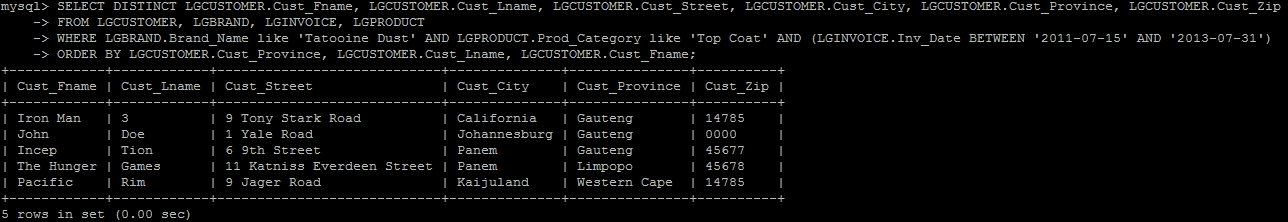
\includegraphics{Queries/Question_8/Q8_screenshot.jpg}
\section {Question 9}
\lstset{
            language=SQL,
            breaklines=true
            }
        \begin{lstlisting}[frame=single]
        SELECT LGEMPLOYEE.Emp_Num, LGEMPLOYEE.Emp_Lname, LGEMPLOYEE.Emp_Email, LGEMPLOYEE.Emp_Title, LGDEPARTMENT.Dept_Name
FROM LGEMPLOYEE INNER JOIN LGDEPARTMENT ON LGEMPLOYEE.Dept_Num=LGDEPARTMENT.Dept_Num
WHERE Emp_Title like '%Associate'
ORDER BY LGDEPARTMENT.Dept_Name, LGEMPLOYEE.Emp_Title;

        \end{lstlisting}
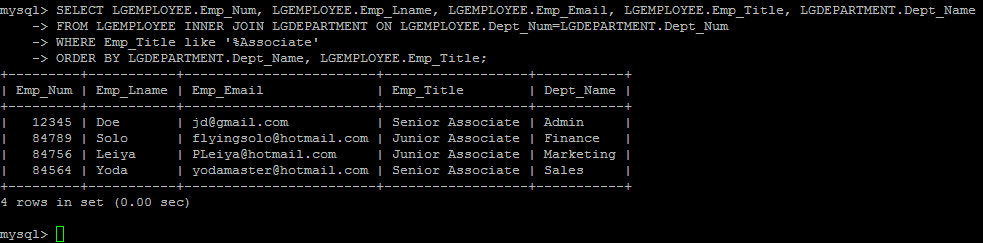
\includegraphics{Queries/Question_9/Question_9_screenshot.PNG}
\maketitle\section {Question 10}
\lstset{
            language=SQL,
            breaklines=true
            }
        \begin{lstlisting}[frame=single]
        SELECT LGBRAND.Brand_Name, COUNT(*) AS 'Amount'
FROM LGPRODUCT JOIN LGBRAND ON LGPRODUCT.Brand_ID=LGBRAND.Brand_ID
GROUP BY LGBRAND.Brand_Name
ORDER BY LGBRAND.Brand_Name;

        \end{lstlisting}
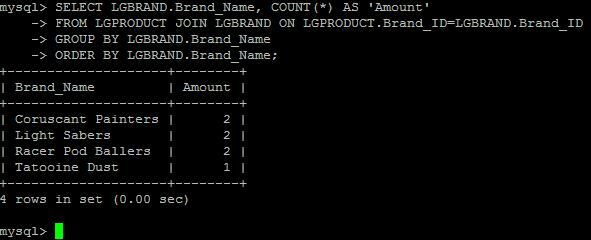
\includegraphics{Queries/Question_10/Question_10_screenshot.PNG}
\section {Question 11}
\lstset{
            language=SQL,
            breaklines=true
            }
        \begin{lstlisting}[frame=single]
        SELECT Prod_Category, COUNT(*) AS 'Amount'
FROM LGPRODUCT
WHERE Prod_Base like 'water'
GROUP BY Prod_Category;

        \end{lstlisting}
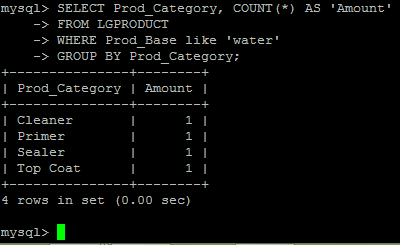
\includegraphics{Queries/Question_11/Question_11_screenshot.PNG}
\section {Question 12}
\lstset{
            language=SQL,
            breaklines=true
            }
        \begin{lstlisting}[frame=single]
        SELECT  Prod_Base, Prod_Type, COUNT(*) AS 'Amount'
FROM LGPRODUCT
GROUP BY Prod_Base, Prod_Type;

        \end{lstlisting}
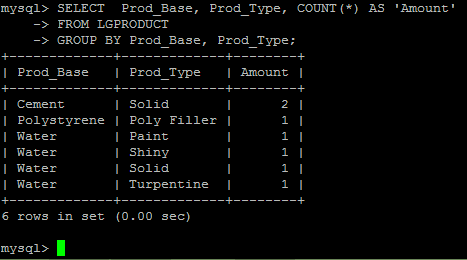
\includegraphics{Queries/Question_12/Question_12_Screenshot.PNG}
\section {Question 13}
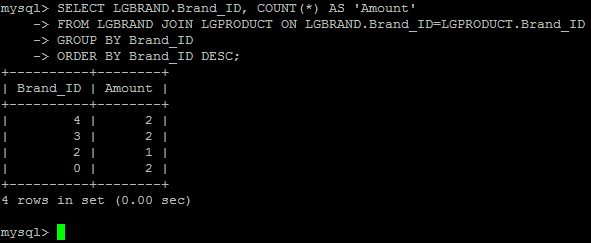
\includegraphics{Queries/Question_13/Question_13_screenshot.PNG}
\lstset{
            language=SQL,
            breaklines=true
            }
        \begin{lstlisting}[frame=single]
        SELECT LGBRAND.Brand_ID, COUNT(*) AS 'Amount'
FROM LGBRAND JOIN LGPRODUCT ON LGBRAND.Brand_ID=LGPRODUCT.Brand_ID
GROUP BY Brand_ID
ORDER BY Brand_ID DESC;

        \end{lstlisting}
\section {Question 14_(17)}
\lstset{
            language=SQL,
            breaklines=true
            }
        \begin{lstlisting}[frame=single]
        SELECT LGPRODUCT.Brand_ID, LGBRAND.Brand_Name, ROUND(AVG(LGPRODUCT.Prod_Price), 2) AS 'Average'
FROM LGBRAND JOIN LGPRODUCT ON LGBRAND.Brand_ID=LGPRODUCT.Brand_ID
GROUP BY LGPRODUCT.Brand_ID
ORDER BY LGBRAND.Brand_Name;

        \end{lstlisting}
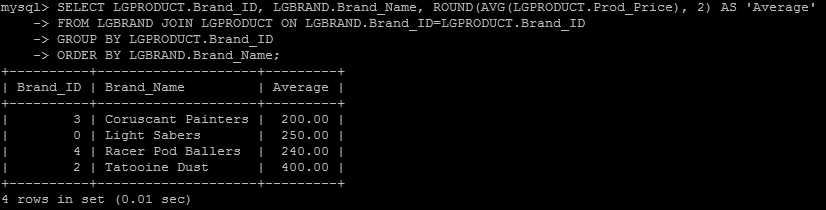
\includegraphics{Queries/Question_14_(17)/Q14_screenshot.jpg}
\section {Question 15_(18)}
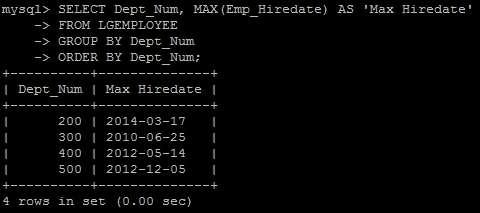
\includegraphics{Queries/Question_15_(18)/Q15_screenshot.jpg}
\lstset{
            language=SQL,
            breaklines=true
            }
        \begin{lstlisting}[frame=single]
        SELECT Dept_Num, MAX(Emp_Hiredate) AS 'Max Hiredate'
FROM LGEMPLOYEE
GROUP BY Dept_Num
ORDER BY Dept_Num;

        \end{lstlisting}
\section {Question 16_(19)}
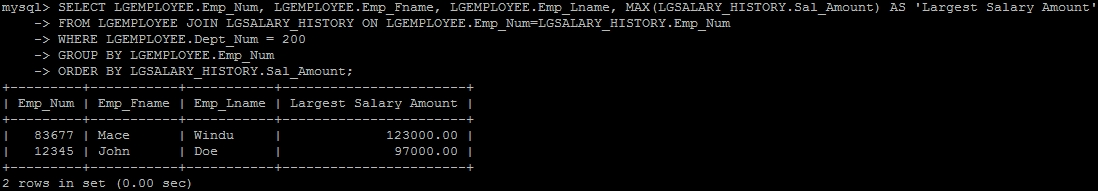
\includegraphics{Queries/Question_16_(19)/Q16_screenshot.jpg}
\lstset{
            language=SQL,
            breaklines=true
            }
        \begin{lstlisting}[frame=single]
        SELECT LGEMPLOYEE.Emp_Num, LGEMPLOYEE.Emp_Fname, LGEMPLOYEE.Emp_Lname, MAX(LGSALARY_HISTORY.Sal_Amount) AS 'Largest Salery Amount'
FROM LGEMPLOYEE JOIN LGSALARY_HISTORY ON LGEMPLOYEE.Emp_Num=LGSALARY_HISTORY.Emp_Num
WHERE LGEMPLOYEE.Dept_Num = 200
GROUP BY LGEMPLOYEE.Emp_Num
ORDER BY LGSALARY_HISTORY.Sal_Amount;

        \end{lstlisting}
\section {Question 20}
\lstset{
            language=SQL,
            breaklines=true
            }
        \begin{lstlisting}[frame=single]
        SELECT LGCUSTOMER.Cust_Code, LGCUSTOMER.Cust_Fname, LGCUSTOMER.Cust_Lname, SUM(LGINVOICE.Inv_Total) AS 'Sum of Invoice Totals'
FROM LGCUSTOMER JOIN LGINVOICE ON LGCUSTOMER.Cust_Code = LGINVOICE.Cust_Code
WHERE LGINVOICE.Inv_Total > 1500
GROUP BY LGINVOICE.Cust_Code
ORDER BY SUM(LGINVOICE.Inv_Total) DESC;

        \end{lstlisting}
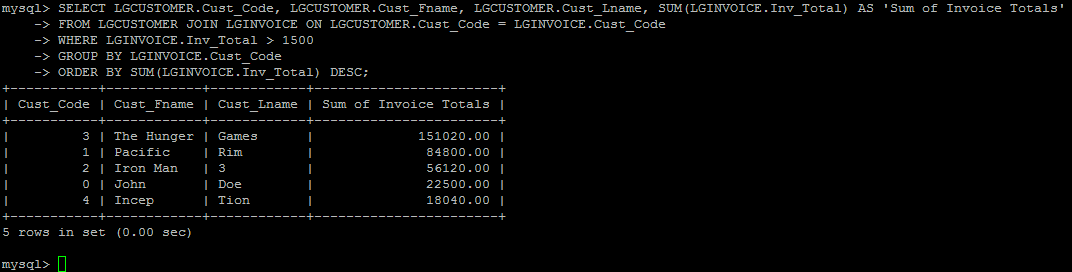
\includegraphics{Queries/Question_20/Question_20_screenshot.PNG}
\section {Question 21}
\lstset{
            language=SQL,
            breaklines=true
            }
        \begin{lstlisting}[frame=single]
        SELECT LGDEPARTMENT.Dept_Num, LGDEPARTMENT.Dept_Name, LGDEPARTMENT.Dept_Phone, LGDEPARTMENT.Emp_Num, LGEMPLOYEE.Emp_Lname
FROM LGDEPARTMENT JOIN LGEMPLOYEE ON LGDEPARTMENT.Emp_Num = LGEMPLOYEE.Emp_Num
WHERE LGEMPLOYEE.Emp_Title like "manager"
ORDER BY LGDEPARTMENT.Dept_Name;

        \end{lstlisting}
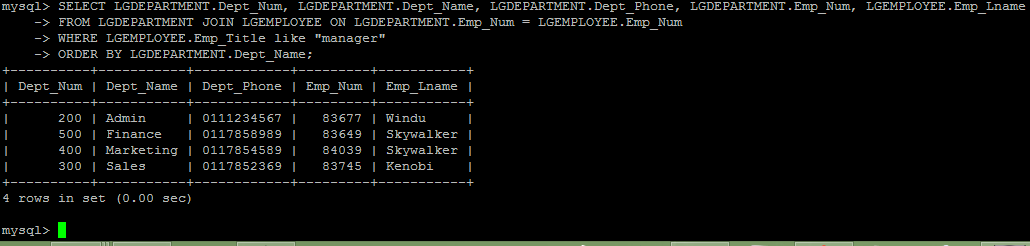
\includegraphics{Queries/Question_21/Question_21_screenshot.PNG}
\section {Question 22}
\lstset{
            language=SQL,
            breaklines=true
            }
        \begin{lstlisting}[frame=single]
        SELECT LGSUPPLIES.Vend_ID, LGVENDOR.Vend_Name, LGBRAND.Brand_Name, COUNT(*) AS 'Amount'
FROM LGVENDOR JOIN (LGSUPPLIES JOIN (LGPRODUCT JOIN LGBRAND ON LGPRODUCT.Brand_ID=LGBRAND.Brand_ID) ON LGSUPPLIES.Prod_SKU=LGPRODUCT.Prod_SKU) ON LGVENDOR.Vend_ID=LGSUPPLIES.Vend_ID
GROUP BY LGSUPPLIES.Vend_ID, LGPRODUCT.Brand_ID
ORDER BY LGVENDOR.Vend_Name, LGBRAND.Brand_Name;
        \end{lstlisting}
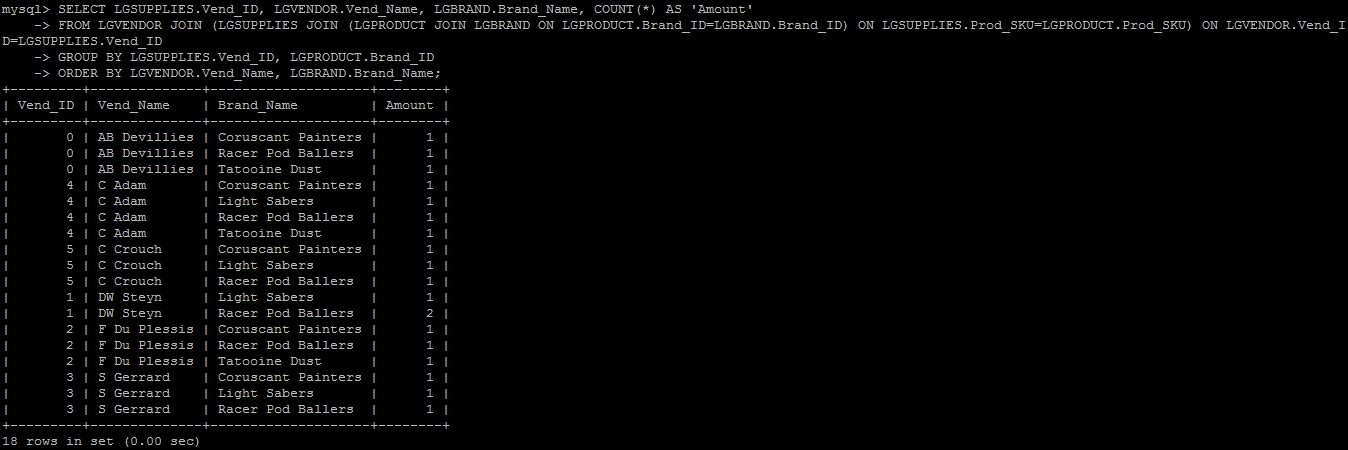
\includegraphics{Queries/Question_22/Q22_screenshot.jpg}
\section {Question 23}
\lstset{
            language=SQL,
            breaklines=true
            }
        \begin{lstlisting}[frame=single]
        select LGEMPLOYEE.Emp_Num, LGEMPLOYEE.Emp_Fname, LGEMPLOYEE.Emp_Lname, sum(LGINVOICE.Inv_Total) as 'Total Invoices' 
from LGEMPLOYEE, LGINVOICE 
where LGEMPLOYEE.Emp_Num = LGINVOICE.Employee_ID group by LGEMPLOYEE.Emp_Num 
order by LGEMPLOYEE.Emp_Fname, LGEMPLOYEE.Emp_Lname;
        \end{lstlisting}
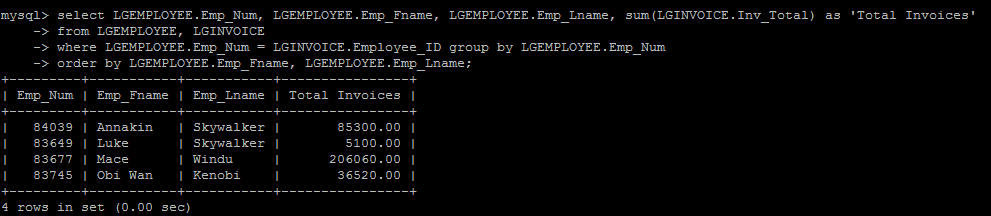
\includegraphics{Queries/Question_23/Question_23_screenshot.PNG}
\section {Question 24}
\lstset{
            language=SQL,
            breaklines=true
            }
        \begin{lstlisting}[frame=single]
        SELECT AVG(Prod_Price) AS 'Largest Average Product Price'
FROM LGPRODUCT
GROUP BY Brand_ID
ORDER BY AVG(Prod_Price) DESC
LIMIT 1;
        \end{lstlisting}
\section {Question 25}
\lstset{
            language=SQL,
            breaklines=true
            }
        \begin{lstlisting}[frame=single]
        #Instead of having two nested queries a HAVING may work better
SELECT Brand_Id, Brand_Name, Brand_Type, MAX(Average_Price_Of_Products) AS 'Max Average Price of Products'
FROM (
	SELECT LGBRAND.Brand_Id, LGBRAND.Brand_Name, LGBRAND.Brand_Type, AVG(LGPRODUCT.Prod_Price) AS 'Average_Price_Of_Products'
	FROM LGBRAND JOIN LGPRODUCT ON LGBRAND.Brand_Id = LGPRODUCT.Brand_Id
	GROUP BY LGBRAND.Brand_Id) Avgerages;

        \end{lstlisting}
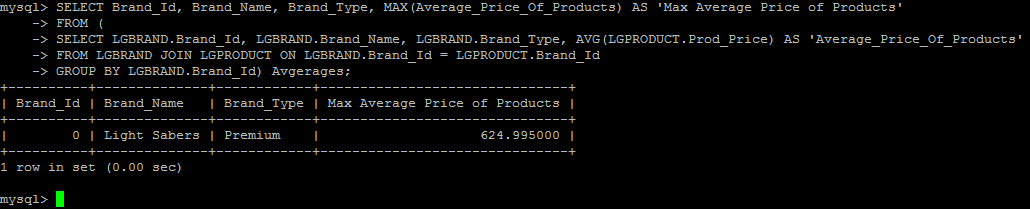
\includegraphics{Queries/Question_25/Question_25_screenshot.PNG}
\section {Question 26}
\lstset{
            language=SQL,
            breaklines=true
            }
        \begin{lstlisting}[frame=single]
        SELECT CONCAT(M.Emp_Fname, ' ', M.Emp_Lname) AS 'Manager_Name', LGDEPARTMENT.Dept_Name, LGDEPARTMENT.Dept_Phone, CONCAT(E.Emp_Fname, ' ', E.Emp_Lname) AS 'Emp_Name', CONCAT(LGCUSTOMER.Cust_Fname, ' ', LGCUSTOMER.Cust_Lname) AS 'Cust_Name', LGINVOICE.Inv_Date, LGINVOICE.Inv_Total
FROM LGCUSTOMER JOIN (LGINVOICE JOIN (LGEMPLOYEE E JOIN (LGDEPARTMENT JOIN LGEMPLOYEE M ON LGDEPARTMENT.Emp_Num=M.Emp_Num) ON E.Dept_Num=LGDEPARTMENT.Dept_Num) ON LGINVOICE.Employee_ID=E.Emp_Num) ON LGCUSTOMER.Cust_Code=LGINVOICE.Cust_Code
WHERE Cust_Lname like 'Doe' AND Inv_Date='2013-03-23';

        \end{lstlisting}
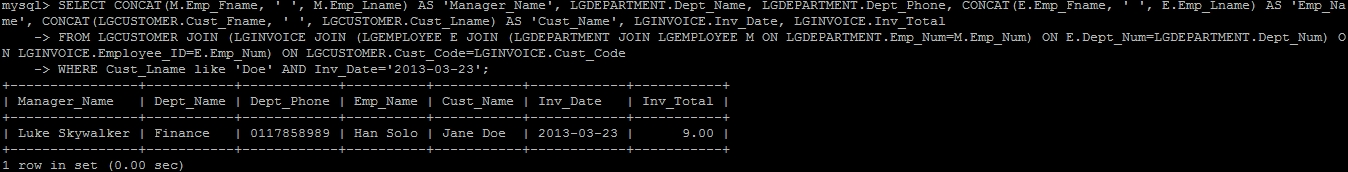
\includegraphics{Queries/Question_26/Q26_screenshot.jpg}
\section {Question 27}
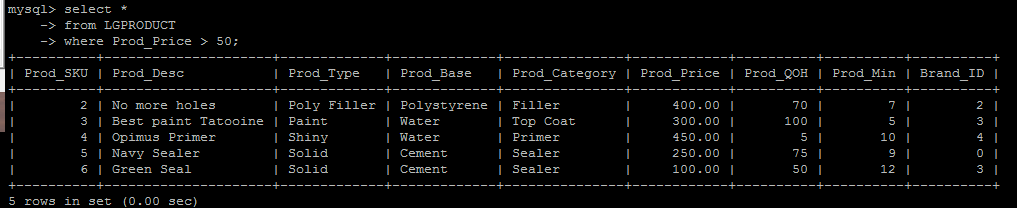
\includegraphics{Queries/Question_27/Question_27_screenshot.PNG}
\lstset{
            language=SQL,
            breaklines=true
            }
        \begin{lstlisting}[frame=single]
        select * 
from LGPRODUCT 
where Prod_Price > 50;
        \end{lstlisting}
\section {Question 28}
\lstset{
            language=SQL,
            breaklines=true
            }
        \begin{lstlisting}[frame=single]
        SELECT LGSALARY_HISTORY.Sal_Amount
FROM LGSALARY_HISTORY JOIN LGEMPLOYEE ON LGSALARY_HISTORY.Emp_Num=LGEMPLOYEE.Emp_Num
WHERE LGEMPLOYEE.Dept_Num=300 AND LGSALARY_HISTORY.Sal_End IS NULL
ORDER BY LGSALARY_HISTORY.Sal_Amount DESC;

        \end{lstlisting}
\section {Question 29}
\lstset{
            language=SQL,
            breaklines=true
            }
        \begin{lstlisting}[frame=single]
        #with this query the earliest Sal_From date is automatically selected.
SELECT Emp_Num, Sal_Amount
FROM LGSALARY_HISTORY
GROUP BY Emp_Num
HAVING MIN(Sal_From)
ORDER BY Emp_Num;

        \end{lstlisting}
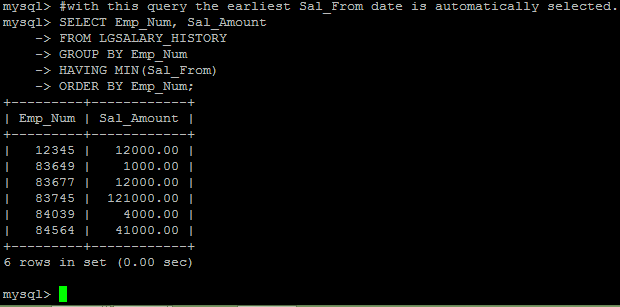
\includegraphics{Queries/Question_29/Question_29_screenshot.PNG}
\section {Question 3}
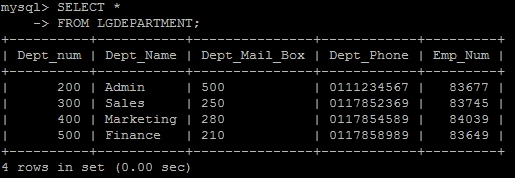
\includegraphics{Queries/Question_3/Q3_screenshot.jpg}
\lstset{
            language=SQL,
            breaklines=true
            }
        \begin{lstlisting}[frame=single]
        SELECT *
FROM LGDEPARTMENT;

        \end{lstlisting}
\section {Question 30}
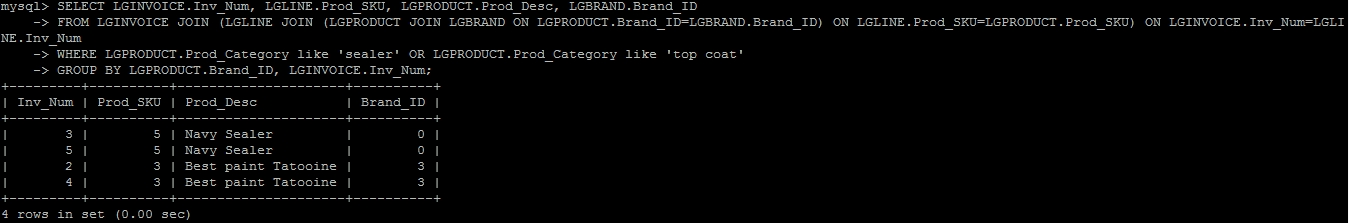
\includegraphics{Queries/Question_30/Q30_screenshot.jpg}
\lstset{
            language=SQL,
            breaklines=true
            }
        \begin{lstlisting}[frame=single]
        SELECT LGINVOICE.Inv_Num, LGLINE.Prod_SKU, LGPRODUCT.Prod_Desc, LGBRAND.Brand_ID
FROM LGINVOICE JOIN (LGLINE JOIN (LGPRODUCT JOIN LGBRAND ON LGPRODUCT.Brand_ID=LGBRAND.Brand_ID) ON LGLINE.Prod_SKU=LGPRODUCT.Prod_SKU) ON LGINVOICE.Inv_Num=LGLINE.Inv_Num
WHERE LGPRODUCT.Prod_Category like 'sealer' OR LGPRODUCT.Prod_Category like 'top coat'
GROUP BY LGPRODUCT.Brand_ID, LGINVOICE.Inv_Num;
        \end{lstlisting}
\section {Question 31}
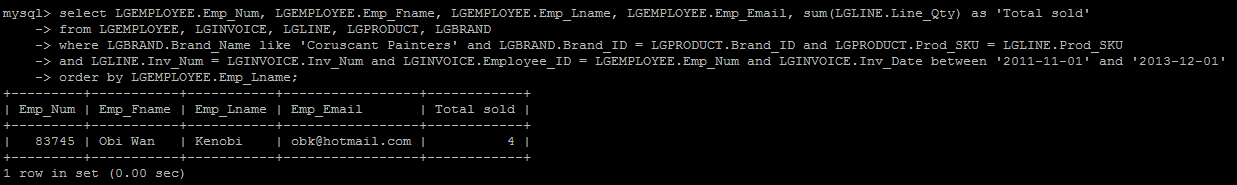
\includegraphics{Queries/Question_31/Question_31_screenshot.PNG}
\lstset{
            language=SQL,
            breaklines=true
            }
        \begin{lstlisting}[frame=single]
        select LGEMPLOYEE.Emp_Num, LGEMPLOYEE.Emp_Fname, LGEMPLOYEE.Emp_Lname, LGEMPLOYEE.Emp_Email, sum(LGLINE.Line_Qty) as 'Total sold' 
from LGEMPLOYEE, LGINVOICE, LGLINE, LGPRODUCT, LGBRAND 
where LGBRAND.Brand_Name like 'Coruscant Painters' and LGBRAND.Brand_ID = LGPRODUCT.Brand_ID and LGPRODUCT.Prod_SKU = LGLINE.Prod_SKU 
and LGLINE.Inv_Num = LGINVOICE.Inv_Num and LGINVOICE.Employee_ID = LGEMPLOYEE.Emp_Num and LGINVOICE.Inv_Date between '2011-11-01' and '2013-12-01' 
order by LGEMPLOYEE.Emp_Lname;
        \end{lstlisting}
\section {Question 32}
\lstset{
            language=SQL,
            breaklines=true
            }
        \begin{lstlisting}[frame=single]
        SELECT L1.Cust_Code, LGCUSTOMER.Cust_Fname, LGCUSTOMER.Cust_Lname
FROM LGINVOICE L1 JOIN (LGCUSTOMER JOIN LGINVOICE L2 ON LGCUSTOMER.Cust_Code=L2.Cust_Code) ON L1.Cust_Code=LGCUSTOMER.Cust_Code
WHERE L1.Employee_ID=83649 AND L2.Employee_ID=83677
ORDER BY LGCUSTOMER.Cust_Lname, LGCUSTOMER.Cust_Fname;

        \end{lstlisting}
\section {Question 33}
\lstset{
            language=SQL,
            breaklines=true
            }
        \begin{lstlisting}[frame=single]
        SELECT LGCUSTOMER.Cust_Code, LGCUSTOMER.Cust_Fname, LGCUSTOMER.Cust_Lname, CONCAT(LGCUSTOMER.Cust_Street, ' ', LGCUSTOMER.Cust_City, ' ', LGCUSTOMER.Cust_Province, ' ', LGCUSTOMER.Cust_ZIP) AS 'Full_Address', LGINVOICE.Inv_Date, MAX(LGINVOICE.Inv_Total) AS 'Largest Invoice'
FROM LGCUSTOMER JOIN LGINVOICE ON LGCUSTOMER.Cust_Code=LGINVOICE.Cust_Code
WHERE LGCUSTOMER.Cust_Province like 'Gauteng'
GROUP BY LGCUSTOMER.Cust_Code;

        \end{lstlisting}
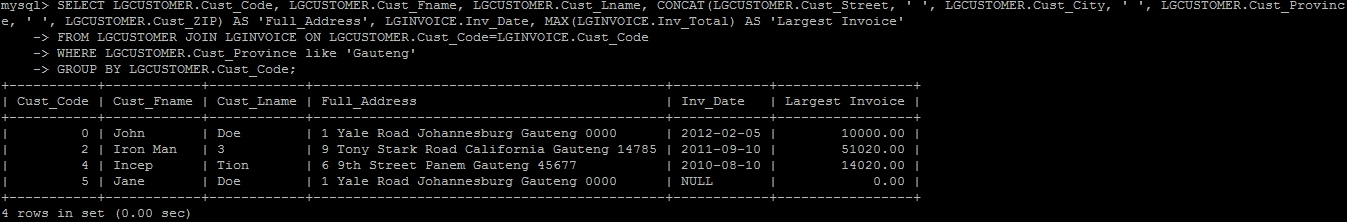
\includegraphics{Queries/Question_33/Q33_screenshot.jpg}
\section {Question 34}
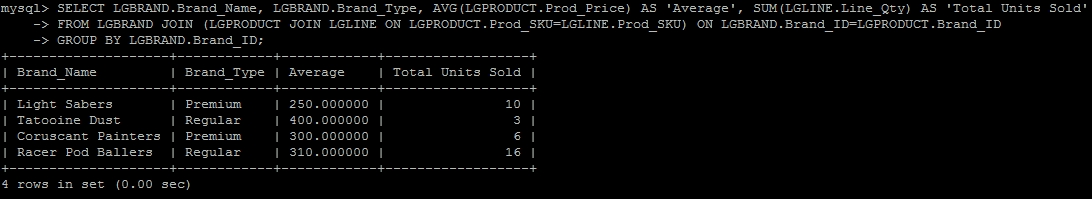
\includegraphics{Queries/Question_34/Q34_screenshot.jpg}
\lstset{
            language=SQL,
            breaklines=true
            }
        \begin{lstlisting}[frame=single]
        SELECT LGBRAND.Brand_Name, LGBRAND.Brand_Type, AVG(LGPRODUCT.Prod_Price) AS 'Average', SUM(LGLINE.Line_Qty) AS 'Total Units Sold'
FROM LGBRAND JOIN (LGPRODUCT JOIN LGLINE ON LGPRODUCT.Prod_SKU=LGLINE.Prod_SKU) ON LGBRAND.Brand_ID=LGPRODUCT.Brand_ID
GROUP BY LGBRAND.Brand_ID;

        \end{lstlisting}
\section {Question 35}
\lstset{
            language=SQL,
            breaklines=true
            }
        \begin{lstlisting}[frame=single]
        select  LGBRAND.Brand_Name, LGBRAND.Brand_Type, LGPRODUCT.Prod_SKU, LGPRODUCT.Prod_Desc, LGPRODUCT.Prod_Price from LGBRAND, LGPRODUCT where LGPRODUCT.Brand_ID = LGBRAND.Brand_ID and  LGBRAND.Brand_Type not like 'Premium' and LGPRODUCT.Prod_Price > (select Max(LGPRODUCT.Prod_Price) from LGPRODUCT, LGBRAND where LGBRAND.Brand_ID = LGPRODUCT.Brand_ID and LGBRAND.Brand_Type like 'Premium');

        \end{lstlisting}
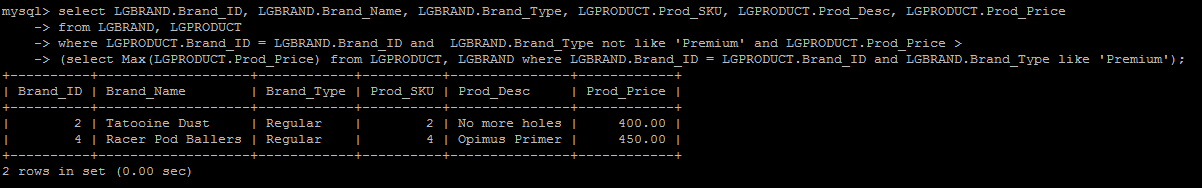
\includegraphics{Queries/Question_35/Question35.PNG}
\end{document}
